\chapter{Kajian Pustaka}
\label{chap:kajian-pustaka}

\section{Deskripsi Permasalahan}
\label{sec:deskripsi-permasalahan}

Sistem monitoring detak jantung berbasis IoT yang ada saat ini umumnya mengadopsi paradigma \textit{cloud-centric}, di mana perangkat sensor hanya bertugas mengumpulkan data fisiologis mentah untuk kemudian dikirimkan ke server pusat guna diproses dan dianalisis. Kondisi ini menyebabkan dua permasalahan mendasar, yaitu latensi sistem yang tinggi akibat \textit{round-trip} data ke server yang dapat mencapai 152,3 ms~\cite{al_quayed_2026}, serta ketidakmampuan sistem untuk beroperasi secara mandiri ketika koneksi jaringan terganggu atau terputus.

Model kecerdasan buatan untuk deteksi aritmia umumnya dijalankan pada perangkat keras desktop atau server, dan baru sedikit yang dibuktikan mampu melakukan inferensi \textit{real-time} pada mikrokontroler \textit{low-power} yang sesungguhnya digunakan dalam perangkat \textit{wearable}~\cite{zambrano_2026}. Pada sisi pengiriman, platform yang mengalirkan sinyal ECG mentah langsung ke server belum menyimpan data secara lokal ketika koneksi terputus, dan mekanisme tersebut masih ditempatkan sebagai pengembangan lanjutan~\cite{escobedo_2026}. Penelitian ini bertujuan untuk mengatasi kedua kesenjangan tersebut melalui implementasi sistem \textit{edge computing} yang mampu menjalankan deteksi aritmia secara \textit{on-device} dengan \textit{pipeline} yang resilien.

\section{Teori Penunjang}
\label{sec:teori-penunjang}

\subsection{Aritmia dan Elektrokardiogram (ECG)}
\label{subsec:aritmia-ecg}

Aritmia merupakan gangguan irama listrik jantung yang menyebabkan detak jantung tidak teratur, terlalu cepat (takikardia), atau terlalu lambat (bradikardia)~\cite{ecg_goldberger}. Kondisi ini dapat dideteksi melalui elektrokardiogram (ECG), yaitu rekaman aktivitas listrik jantung yang menangkap gelombang P, kompleks QRS, dan gelombang T dalam satu siklus detak jantung~\cite{ecg_goldberger}. Penyimpangan morfologi atau durasi pada komponen-komponen tersebut menjadi penanda klinis adanya aritmia. Dalam implementasi \textit{wearable}, sinyal ECG rentan terhadap tiga jenis gangguan utama, yaitu \textit{baseline wander} (frekuensi $< 0{,}5$ Hz), \textit{high-frequency noise} ($> 40$ Hz), serta \textit{muscle artifact} dan \textit{motion artifact}~\cite{zambrano_2026, jia_2024}. \textit{Muscle artifact} yang berasal dari aktivitas listrik otot paling sulit ditangani karena sifatnya tidak stasioner dan spektrum frekuensinya tumpang tindih dengan sinyal ECG ($0{,}5$--$40$ Hz)~\cite{jia_2024}.
% sumber: jia_2024 (PMC11591354) "The identification of EMG noise presents a greater challenge compared to PLI and BW noises, given its non-stationary nature and substantial overlaps across entire frequency bands with ECG data"; daftar singkatan: MAs = Muscle Artifacts, EMs = Electrode Motion Artifacts

Tabel~\ref{tab:perbandingan-irama} merangkum perbedaan karakteristik
sinyal ECG antara irama sinus normal dan kondisi aritmia yang menjadi
dasar klasifikasi pada penelitian ini.

\begin{table}[!ht]
  \centering
  \caption{Perbandingan karakteristik irama sinus normal dan aritmia
           pada sinyal ECG}
  \label{tab:perbandingan-irama}
  \small
  \begin{tabular}{p{3.0cm}p{4.5cm}p{4.5cm}}
    \toprule
    \textbf{Karakteristik} &
    \textbf{Irama Sinus Normal} &
    \textbf{Aritmia} \\
    \midrule
    Gelombang P &
    Terlihat jelas dan reguler sebelum setiap kompleks QRS &
    Tidak ada, tidak teratur, atau bermorfologi abnormal \\
    Kompleks QRS &
    Sempit ($<$120 ms), morfologi konsisten antardetak &
    Dapat melebar ($>$120 ms) atau bermorfologi bervariasi \\
    Interval R-R &
    Teratur, variasi antardetak kecil &
    Tidak teratur atau menunjukkan fluktuasi besar \\
    Laju jantung &
    60--100 bpm &
    Di bawah 60 bpm (bradikardia) atau di atas 100 bpm (takikardia) \\
    Gelombang T &
    Positif dan konsisten pada sadapan II &
    Dapat terbalik atau berubah bentuk \\
    \bottomrule
  \end{tabular}
  \smallskip\\
  \small\textbf{Sumber: Goldberger~\cite{ecg_goldberger}}
\end{table}

Dalam penelitian ini, perbedaan karakteristik pada
Tabel~\ref{tab:perbandingan-irama} digunakan sebagai landasan klasifikasi
biner Normal dan Aritmia pada pemetaan anotasi dataset MIT-BIH.

\subsection{Filter Butterworth}
\label{subsec:teori-butterworth}

Filter Butterworth merupakan filter yang memiliki respons amplitudo datar pada pita lolos tanpa riak. Karakteristik tersebut mempertahankan komponen sinyal di dalam pita yang dipilih dan meredam komponen di luarnya secara bertahap~\cite{bui_2021}. Filter \textit{bandpass} dibentuk dengan menggabungkan batas bawah dan batas atas agar hanya rentang frekuensi yang dibutuhkan yang diteruskan. Pada ECG, batas bawah mengurangi \textit{baseline wander}, sedangkan batas atas meredam gangguan berfrekuensi tinggi~\cite{zambrano_2026, bui_2021}.

Filter digital berorde tinggi dapat direalisasikan sebagai rangkaian \textit{second-order section} atau \textit{biquad}. Bentuk ini memecah fungsi transfer menjadi beberapa bagian berorde dua dan mengurangi kepekaan perhitungan terhadap pembulatan koefisien. Pemrosesan kausal menghasilkan keluaran dari sampel saat ini dan sampel sebelumnya sehingga dapat dijalankan sampel demi sampel secara \textit{real-time}. Konsekuensinya adalah \textit{group delay} yang menggeser posisi fitur sinyal terhadap masukan. Dalam penelitian ini, filter Butterworth \textit{bandpass} digunakan untuk mempertahankan pita ECG 0,5--40 Hz sebelum deteksi R-\textit{peak} dan klasifikasi pada ESP32-S3.

\subsection{Algoritma Pan-Tompkins}
\label{subsec:teori-pan-tompkins}

Algoritma Pan-Tompkins merupakan metode deteksi kompleks QRS secara \textit{real-time} yang mengubah sinyal ECG menjadi deret puncak energi~\cite{pan_tompkins_1985}. Tahap \textit{bandpass} menekan pergeseran garis dasar dan gangguan di luar pita QRS. Operasi turunan kemudian menonjolkan kemiringan tajam, sedangkan pengkuadratan membuat seluruh nilai positif dan memperbesar perbedaan antara kompleks QRS dan komponen beramplitudo kecil. Integrasi jendela bergerak menggabungkan informasi kemiringan dan lebar menjadi satu bentuk pulsa yang dapat dibandingkan dengan ambang.

Ambang Pan-Tompkins diperbarui dari estimasi tingkat sinyal dan gangguan agar detektor mengikuti perubahan amplitudo ECG~\cite{pan_tompkins_1985, li_2020}. Sesudah satu puncak diterima, periode refraktori mencegah kompleks QRS yang sama dihitung lebih dari sekali. Nilai refraktori yang terlalu panjang dapat menahan detak prematur, sedangkan nilai yang terlalu pendek meningkatkan risiko deteksi ganda. Dalam penelitian ini, Pan-Tompkins digunakan untuk menentukan lokasi R-\textit{peak} sebagai acuan segmentasi detak dan perhitungan interval R-R.

\subsection{Indeks Kualitas Sinyal ECG}
\label{subsec:teori-sqi}

Indeks kualitas sinyal ECG atau \textit{signal quality index} (SQI) menilai apakah sinyal cukup layak untuk dianalisis tanpa memerlukan label irama klinis. Pendekatan berbasis aturan memeriksa kelayakan fisiologis detak dan konsistensi morfologi kompleks QRS pada potongan waktu tertentu~\cite{syversen_2024}. Penilaian per jendela mencegah bagian sinyal yang buruk tertutupi oleh ringkasan satu rekaman penuh.

SQI yang digunakan terdiri atas empat pemeriksaan. Tiga pemeriksaan fisiologis mensyaratkan laju jantung 40 sampai 180 detak per menit, jarak antar-R-\textit{peak} paling lama 3 detik, serta rasio interval R-R terpanjang terhadap terpendek di bawah 2,2~\cite{syversen_2024}. Pemeriksaan morfologi memotong kompleks QRS di sekitar setiap R-\textit{peak}, membentuk \textit{template} dari rerata potongan, lalu menghitung korelasi setiap potongan terhadap \textit{template}. Jendela dinilai layak apabila rerata korelasinya minimal 0,66. Dalam penelitian ini, SQI diterapkan pada jendela 10 detik untuk menilai kelayakan rekaman tubuh sebagai masukan jalur preprocessing.

\subsection{Algoritma Goertzel}
\label{subsec:teori-goertzel}

Algoritma Goertzel menghitung satu komponen frekuensi dari sekumpulan sampel tanpa membentuk seluruh spektrum~\cite{goertzel_1958}. Perhitungan ini menggunakan relasi rekursif orde dua pada Persamaan~\ref{eq:goertzel-rekursif}.

\begin{equation}
\label{eq:goertzel-rekursif}
s[n] = x[n] + 2\cos(\omega_0)s[n-1] - s[n-2]
\end{equation}

\noindent di mana $x[n]$ adalah sampel masukan, $s[n]$ adalah keadaan rekursif, dan $\omega_0$ adalah frekuensi sudut yang diperiksa. Setelah seluruh sampel diproses, magnitudo komponen diperoleh dari dua keadaan terakhir. Kebutuhan memori metode ini tetap kecil karena tidak menyimpan seluruh keluaran transformasi frekuensi. Dalam penelitian ini, Goertzel digunakan untuk mengukur amplitudo dengung jala-jala 50 Hz setiap detik sebagai bagian dari penilaian kontak elektroda.

\subsection{IoT Edge Computing}
\label{subsec:iot-edge}

IoT \textit{edge computing} adalah pendekatan arsitektur yang menempatkan kapabilitas komputasi langsung pada perangkat \textit{edge}, alih-alih mengandalkan server terpusat. Dengan paradigma ini, data diproses secara lokal sehingga latensi berkurang dan privasi data lebih terjaga~\cite{cao_2020}. Data yang diproses di perangkat juga tetap dapat dipertahankan ketika koneksi internet terputus~\cite{yaacoub_2020}. Arsitektur yang umum digunakan terdiri dari tiga lapisan, yaitu lapisan perangkat (\textit{device layer}) untuk akuisisi dan pemrosesan lokal, lapisan \textit{edge/fog} untuk agregasi, serta lapisan \textit{cloud} untuk penyimpanan dan pemantauan jangka panjang. Dalam konteks monitoring kesehatan, \textit{edge computing} memungkinkan perangkat \textit{wearable} menghasilkan diagnosis secara \textit{real-time} tanpa harus mengirimkan seluruh data mentah ke \textit{cloud}~\cite{tinyml_iot_review}. Dalam penelitian ini, \textit{edge computing} digunakan untuk menempatkan preprocessing dan klasifikasi aritmia pada lapisan perangkat, yaitu ESP32-S3, sedangkan lapisan \textit{cloud} berperan untuk pemantauan dan penyimpanan hasil.

\subsection{Tiny Machine Learning (TinyML)}
\label{subsec:tinyml}

TinyML adalah subdisiplin \textit{machine learning} yang berfokus pada
\textit{deployment} model inferensi pada perangkat dengan sumber daya
terbatas, yaitu mikrokontroler dengan konsumsi daya sekitar 1 mW serta RAM,
prosesor, dan catu daya yang terbatas~\cite{tinyml_iot_review}.
% sumber: laporan/pustaka/tinyml_iot_review.pdf ("typically, these devices consume around one mW"; "limitations of volatile memory (RAM), processing capacity (CPU), and power requirements of microcontrollers") TinyML memungkinkan model kecerdasan buatan
dijalankan langsung pada perangkat \textit{edge} tanpa membutuhkan koneksi ke
server, sehingga mendukung pengambilan keputusan secara \textit{real-time} dan
mandiri. \textit{Framework} yang umum digunakan meliputi TensorFlow Lite for
Microcontrollers (TFLite Micro), Edge Impulse, dan CMSIS-NN. Dalam
penelitian ini, TinyML digunakan untuk menjalankan model deteksi aritmia
pada ESP32-S3 melalui TFLite Micro.

\subsection{Jaringan Saraf Konvolusional Satu Dimensi (1D-CNN)}
\label{subsec:cnn-1d}

Jaringan saraf konvolusional (\textit{Convolutional Neural Network}, CNN)
adalah arsitektur \textit{deep learning} yang secara otomatis mengekstrak fitur
hierarkis dari data masukan melalui operasi konvolusi, tanpa memerlukan
rekayasa fitur manual~\cite{kim_2023}. Pada sinyal satu dimensi seperti ECG,
digunakan varian 1D-CNN yang mengoperasikan \textit{kernel} sepanjang dimensi
waktu untuk menangkap pola morfologi lokal seperti kompleks QRS, gelombang P,
dan gelombang T~\cite{kiranyaz_2021}.

Operasi inti konvolusi 1D pada setiap posisi $t$ dituliskan pada Persamaan~\ref{eq:conv1d}.

\begin{equation}
\label{eq:conv1d}
y[t] = \text{ReLU}\!\left(\sum_{k=0}^{K-1} w[k] \cdot x[t+k] + b\right)
\end{equation}

di mana $x$ adalah sinyal masukan (segmen ECG), $w$ adalah bobot
\textit{kernel} berukuran $K$, $b$ adalah bias, dan $y$ adalah nilai peta
fitur (\textit{feature map}) setelah aktivasi ReLU. Setiap \textit{kernel}
belajar mengenali satu pola lokal tertentu. Dengan banyak \textit{kernel}
yang dilatih secara paralel, CNN dapat menangkap beragam karakteristik
morfologi sekaligus.

Keunggulan utama 1D-CNN untuk klasifikasi ECG dibandingkan metode
berbasis ekstraksi fitur manual (seperti SVM berbasis HRV) adalah
kemampuannya belajar langsung dari sinyal mentah tanpa memerlukan pengetahuan
pakar untuk merancang fitur secara manual~\cite{mekhfioui_2025}. Selain itu, arsitektur yang menggunakan \textit{Global Average Pooling} (GAP) sebagai pengganti
lapisan \textit{flatten} dapat menekan jumlah parameter secara berarti~\cite{mekhfioui_2025},
menjadikan model berukuran kecil. Ukuran model yang ringkas inilah yang
memungkinkan inferensi 1D-CNN terkuantisasi dijalankan langsung pada mikrokontroler
berdaya rendah~\cite{kim_2023}. Pada tahap penerapan di perangkat, operasi GAP dapat
diwujudkan oleh operasi lain yang setara secara matematis apabila \textit{runtime}
mikrokontroler tidak menghitungnya dengan benar. Dalam penelitian ini, 1D-CNN digunakan sebagai
cabang morfologi model deteksi aritmia yang membaca segmen ECG di sekitar puncak R,
dan dilengkapi cabang ritme berbasis interval R-R.

\subsection{Kuantisasi Model CNN}
\label{subsec:kuantisasi}

Kuantisasi adalah teknik kompresi model \textit{neural network} yang mengubah
representasi numerik bobot dari \textit{floating-point} 32-bit (float32) menjadi
\textit{integer} 8-bit (INT8). Teknik ini menghasilkan pengurangan ukuran model
hingga $4\times$ dengan penurunan akurasi yang kecil~\cite{jacob_2018}. Kuantisasi menjadi teknik krusial dalam
TinyML karena memungkinkan model CNN yang semula terlalu besar untuk memori
MCU dapat di-\textit{deploy} pada ESP32-S3 (512 KB SRAM internal). Pemetaan bobot \textit{float32} ke INT8 pada kuantisasi dituliskan pada Persamaan~\ref{eq:kuantisasi}.

\begin{equation}
\label{eq:kuantisasi}
w_\text{int8} = \text{round}\!\left(\frac{w_\text{float32}}{\text{scale}}\right)
+ \text{zero\_point}
\end{equation}

\noindent di mana $w_\text{int8}$ adalah bobot hasil kuantisasi dalam format
INT8 dan $w_\text{float32}$ adalah bobot asli dalam format float32.
\textit{Scale} adalah faktor skala yang memetakan rentang nilai float32 ke
rentang INT8, sedangkan \textit{zero\_point} adalah nilai offset yang memastikan
angka nol pada float32 terpetakan secara tepat ke bilangan bulat pada INT8.

Dalam penelitian ini, kuantisasi digunakan untuk mengecilkan model CNN
menjadi INT8 melalui \textit{post-training quantization} bawaan TensorFlow
Lite. Hasilnya berupa model berformat \textit{FlatBuffer} (.h) yang langsung
dapat dikompilasi bersama \textit{firmware} ESP32-S3 menggunakan TFLite Micro.

\subsection{Mikrokontroler ESP32-S3}
\label{subsec:esp32}

ESP32-S3 adalah mikrokontroler 32-bit dari Espressif Systems dengan prosesor \textit{dual-core} Xtensa LX7, instruksi vektor (SIMD) untuk mempercepat algoritma kecerdasan buatan, serta WiFi dan Bluetooth LE terintegrasi~\cite{espressif_esp32s3_datasheet}. \textit{Board} yang digunakan adalah \textit{board} kompatibel ESP32-S3-DevKitC-1 dengan modul ESP32-S3-WROOM-1-N16R8, yaitu modul dengan memori Flash 16 MB dan PSRAM 8 MB~\cite{espressif_esp32s3_wroom1}. Spesifikasi modul tersebut dirangkum pada Tabel~\ref{tab:spesifikasi-esp32}, dan \textit{board}-nya ditunjukkan pada Gambar~\ref{fig:esp32}.

\begin{table}[!ht]
  \centering
  \caption{Spesifikasi Modul ESP32-S3-WROOM-1-N16R8}
  \label{tab:spesifikasi-esp32}
  \small
  \begin{tabularx}{\linewidth}{>{\RaggedRight\arraybackslash}p{3.6cm}>{\RaggedRight\arraybackslash}X}
    \toprule
    \textbf{Parameter} & \textbf{Spesifikasi} \\
    \midrule
    Prosesor & Xtensa LX7 32-bit \textit{dual-core}, hingga 240 MHz, dengan FPU \\
    Akselerasi & Instruksi vektor (SIMD) 128 bit \\
    Memori internal & ROM 384 KB, SRAM 512 KB, RTC SRAM 16 KB \\
    Flash & 16 MB, Quad SPI \\
    PSRAM & 8 MB, Octal SPI \\
    WiFi & IEEE 802.11 b/g/n, 2,4 GHz \\
    Bluetooth & Bluetooth LE 5 \\
    ADC & 2 ADC SAR 12 bit, hingga 20 kanal \\
    GPIO & 36 pin pada modul, 33 dapat dipakai \\
    Antarmuka & UART, I2C, I2S, SPI, LED PWM 8 kanal, RMT, USB OTG, USB Serial/JTAG \\
    Tegangan kerja modul & 3,0--3,6 V \\
    Suhu operasi & $-$40 sampai 65~$^{\circ}$C \\
    \bottomrule
  \end{tabularx}
  \par\vspace{2pt}{\footnotesize\raggedright Keterangan: tiga pin GPIO dipakai PSRAM Octal SPI, sehingga dari 36 pin modul tersisa 33 pin.\par}
  \smallskip
  {\footnotesize Sumber: Espressif Systems~\cite{espressif_esp32s3_datasheet, espressif_esp32s3_wroom1}\par}
\end{table}
% sumber: ESP32-S3 Series Datasheet v2.2 hlm. 3-5, 36-39, 58-59 (LX7 240 MHz, SIMD 128-bit PIE, ROM 384/SRAM 512/RTC 16 KB, 2x SAR 12-bit 20 kanal, ADC2 tidak bersama Wi-Fi, antarmuka); ESP32-S3-WROOM-1 Datasheet v1.8 Tabel 1-1 hlm. 3 (N16R8: 16 MB Quad SPI flash, 8 MB Octal SPI PSRAM, -40..65 C), hlm. 2 dan 12 (36 GPIO, IO35-37 untuk PSRAM octal), Tabel 6-2 hlm. 27 (VDD33 3,0-3,6 V)

\begin{figure}[!ht]
  \centering
  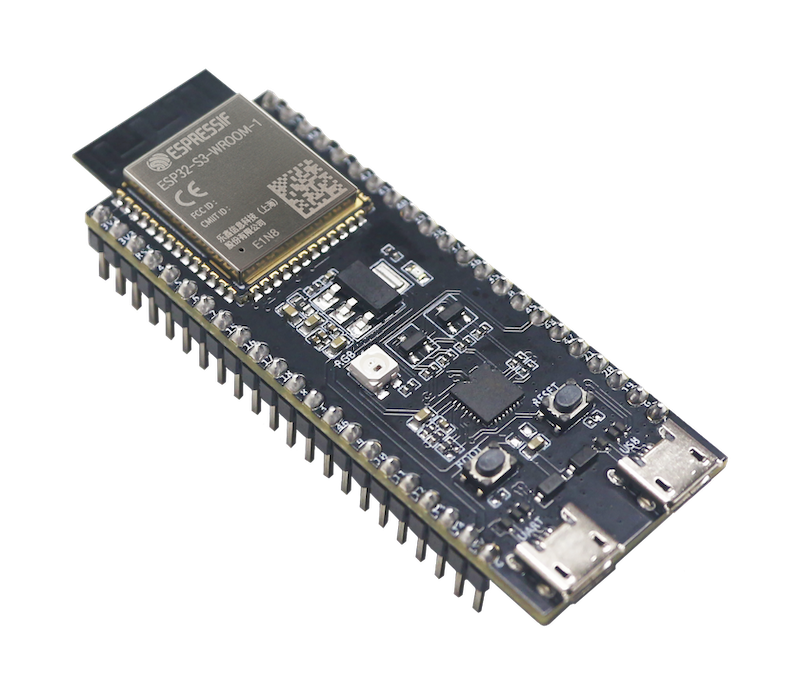
\includegraphics[width=0.5\linewidth,keepaspectratio]{gambar/esp32s3_devkitc1.png}
  \caption[\textit{Board} ESP32-S3-DevKitC-1]{\textit{Board} ESP32-S3-DevKitC-1~\cite{espressif_devkitc1}}
  \label{fig:esp32}
\end{figure}
% sumber gambar: https://docs.espressif.com/projects/esp-dev-kits/en/latest/esp32s3/_images/esp32-s3-devkitc-1-v1.1-isometric.png

ESP32-S3 menjadi satu-satunya perangkat \textit{edge} dalam penelitian ini dan menjalankan akuisisi sinyal AD8232, preprocessing, inferensi model INT8 melalui TensorFlow Lite for Microcontrollers, dan pengiriman MQTT. ESP32-S3 dipilih karena SRAM 512 KB jauh melebihi kebutuhan model INT8 sekitar 23 KB beserta \textit{tensor arena} sekitar 13 KB, PSRAM 8 MB dapat menampung antrean data selama koneksi terputus, dan WiFi sudah terintegrasi. Inferensi 1D-CNN INT8 bahkan telah berjalan pada mikrokontroler yang SRAM-nya jauh lebih kecil, seperti ARM Cortex-M4~\cite{kim_2023, sheeba_rani_2026} dan Arduino UNO 8-bit~\cite{zambrano_2026}. Sinyal AD8232 dicuplik melalui kanal ADC pertama karena ADC kedua tidak dapat dipakai bersamaan dengan WiFi~\cite{espressif_esp32s3_datasheet}.
% sumber: model/artifacts/metrics/fase7_delta.csv (ukuran_kb 22.94); model/CLAUDE.md HW-1 (arena 12.948 B), HW-6 (backlog 27.000 beat di PSRAM); firmware/include/perangkat.h (KANAL_EKG = ADC1_CHANNEL_0)

\subsection{Modul Sensor AD8232}
\label{subsec:ad8232}

AD8232 adalah \textit{front-end} analog terintegrasi untuk akuisisi sinyal ECG \textit{single-lead}. Chip ini memuat penguat instrumentasi \textit{low-noise}, filter \textit{high-pass} untuk meredam \textit{baseline wander}, filter \textit{low-pass} untuk meredam \textit{high-frequency noise}, serta deteksi lepasnya elektroda (\textit{lead-off detection})~\cite{analog_ad8232}. Keluarannya berupa sinyal analog yang dapat dicuplik langsung oleh ADC mikrokontroler. Modul AD8232 beserta elektrodanya ditunjukkan pada Gambar~\ref{fig:ad8232}.

\begin{figure}[!ht]
  \centering
  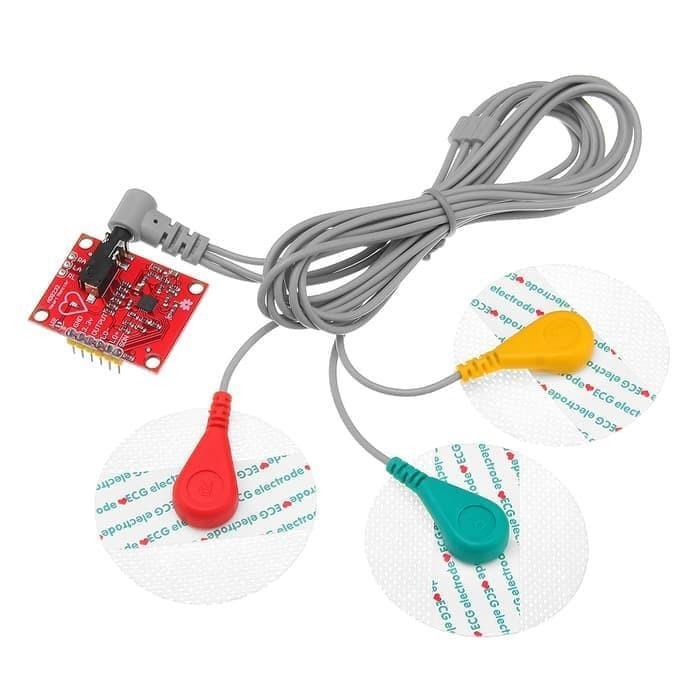
\includegraphics[width=0.55\linewidth,keepaspectratio]{gambar/gambar_2_2.png}
  \caption{Modul sensor AD8232 beserta elektroda \textit{wet-gel} tiga sadapan}
  \label{fig:ad8232}
\end{figure}

Dalam penelitian ini, AD8232 digunakan untuk menangkap sinyal ECG melalui tiga elektroda pada sadapan \textit{Modified Lead II} (MLII), karena gelombang R pada sadapan ini paling tinggi sehingga andal untuk deteksi R-\textit{peak}. Modul ini dipilih karena penguatan dan penyaringan sinyalnya sudah terintegrasi, keluarannya dapat langsung dicuplik ADC ESP32-S3, dan modul yang sama dipakai pada penelitian terkait yang menjadi pembanding~\cite{zambrano_2026, mulyawan_2026}.

\subsection{Layar TFT ST7789}
\label{subsec:tft-st7789}

ST7789 adalah \textit{controller} sekaligus \textit{driver} tunggal untuk layar TFT LCD 262 ribu warna dengan memori bingkai (\textit{frame memory}) internal berukuran 240$\times$320 piksel, sehingga mikrokontroler hanya perlu mengirim data piksel untuk area yang berubah. Chip ini menerima data melalui antarmuka paralel, RGB, maupun SPI tiga atau empat jalur~\cite{sitronix_st7789v3}. Contoh modul layar TFT 1,47 inci dengan \textit{driver} ST7789 ditunjukkan pada Gambar~\ref{fig:tft-st7789}.

\begin{figure}[!ht]
  \centering
  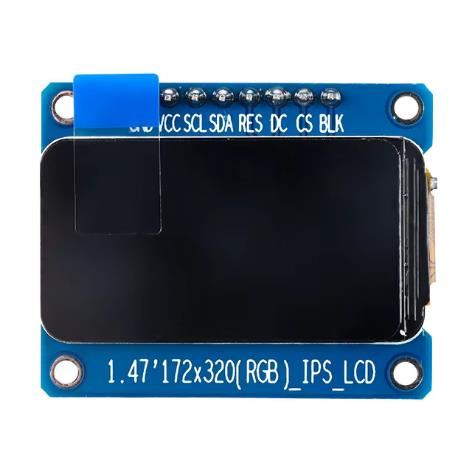
\includegraphics[width=0.4\linewidth,keepaspectratio]{gambar/modul_tft_st7789_mulyawan.png}
  \caption[Modul layar TFT 1,47 inci dengan \textit{driver} ST7789]{Modul layar TFT 1,47 inci dengan \textit{driver} ST7789~\cite{mulyawan_2026}}
  \label{fig:tft-st7789}
\end{figure}
% sumber gambar: Gambar 2.6 buku PA Mulyawan 2026 (pdfimages hlm. 43, 472x472 px)

Dalam penelitian ini, layar TFT 1,47 inci beresolusi 172$\times$320 piksel dengan \textit{driver} ST7789 digunakan untuk menampilkan laju jantung, gelombang ECG, waktu, status perekaman, dan menu. Layar ini dipilih karena ukurannya ringkas untuk perangkat yang dikenakan, resolusinya cukup untuk menampilkan gelombang ECG, dan antarmuka SPI hanya membutuhkan sedikit pin.

\subsection{Modul \textit{Buzzer} Pasif}
\label{subsec:buzzer-pasif}

\textit{Buzzer} pasif, atau \textit{buzzer} transduser, tidak memiliki rangkaian penggerak internal sehingga harus digerakkan gelombang kotak dari luar, dan frekuensi bunyinya mengikuti frekuensi gelombang tersebut. Sebaliknya, \textit{buzzer} aktif atau \textit{buzzer} indikator berbunyi pada satu frekuensi tetap begitu diberi tegangan searah~\cite{cui_buzzer_basics}. Contoh modul \textit{buzzer} pasif tiga pin dengan transistor penggerak ditunjukkan pada Gambar~\ref{fig:buzzer-pasif}.

\begin{figure}[!ht]
  \centering
  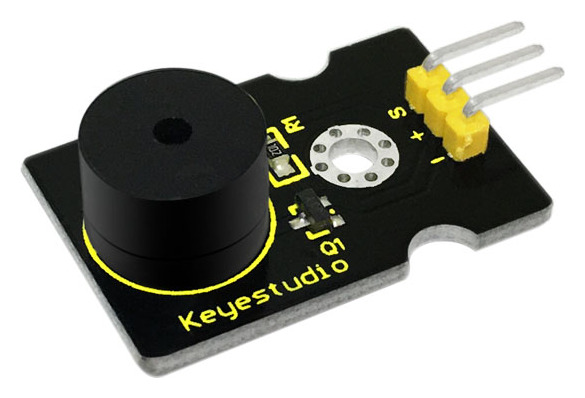
\includegraphics[width=0.45\linewidth,keepaspectratio]{gambar/modul_buzzer_pasif.jpg}
  \caption[Modul \textit{buzzer} pasif tiga pin]{Modul \textit{buzzer} pasif tiga pin~\cite{keyestudio_ks0019}}
  \label{fig:buzzer-pasif}
\end{figure}
% sumber gambar: https://wiki.keyestudio.com/images/a/af/KS0019_%284%29.jpg (dipotong tepinya)

Dalam penelitian ini, modul \textit{buzzer} pasif tiga pin dengan transistor penggerak digunakan sebagai indikator bunyi. \textit{Buzzer} pasif dipilih karena gelombang kotaknya dapat dibangkitkan periferal PWM ESP32-S3, sehingga nada dapat diatur dan satu bip dapat dibunyikan untuk setiap detak.

\subsection{Protokol MQTT}
\label{subsec:mqtt}

MQTT (\textit{Message Queuing Telemetry Transport}) adalah protokol komunikasi \textit{publish-subscribe} yang dirancang untuk perangkat IoT dengan \textit{overhead} \textit{header} minimal (2 byte) sehingga efisien dalam penggunaan \textit{bandwidth}~\cite{oasis_mqtt5}. MQTT mendukung tiga tingkat \textit{Quality of Service}, yaitu QoS-0 (\textit{at most once}), QoS-1 (\textit{at least once}), dan QoS-2 (\textit{exactly once}). Pada aplikasi kesehatan berbasis MQTT, QoS-1 menjadi kompromi terbaik antara latensi \textit{end-to-end} yang rendah dan variasi latensi yang kecil~\cite{akshatha_2022}. Dalam penelitian ini, MQTT digunakan untuk mengirim hasil klasifikasi per detak dari ESP32-S3 ke \textit{broker} ThingsBoard pada QoS-1, dan duplikat akibat pengiriman ulang dikenali di sisi \textit{cloud}.

\subsection{Platform Dashboard ThingsBoard}
\label{subsec:thingsboard}

ThingsBoard adalah platform IoT \textit{open-source} yang menyediakan
infrastruktur lengkap untuk pengumpulan, pemrosesan, visualisasi, dan
manajemen data perangkat IoT. Platform ini mendukung penerimaan data dari
perangkat melalui protokol MQTT secara langsung, menyimpannya dalam basis
data telemetri, dan menampilkannya melalui \textit{dashboard} yang dapat
dikonfigurasi sepenuhnya~\cite{reoukadji_2025}.

ThingsBoard Community Edition (CE) dapat di-\textit{host} secara mandiri
(\textit{self-hosted}). Arsitekturnya terdiri dari tiga komponen utama, yaitu
\textit{broker} MQTT terintegrasi yang menerima data telemetri dari perangkat,
mesin penyimpanan telemetri berbasis \textit{time-series} untuk rekaman
historis, dan \textit{dashboard engine} berbasis WebSocket. \textit{Dashboard
engine} memperbarui tampilan secara otomatis setiap paket baru diterima
sehingga menghasilkan perilaku \textit{real-time} dengan interval pembaruan
$\approx$1 detik tanpa perlu \textit{refresh} halaman. Tampilan antarmuka
ThingsBoard CE ditunjukkan pada Gambar~\ref{fig:thingsboard}.

\begin{figure}[H]
  \centering
  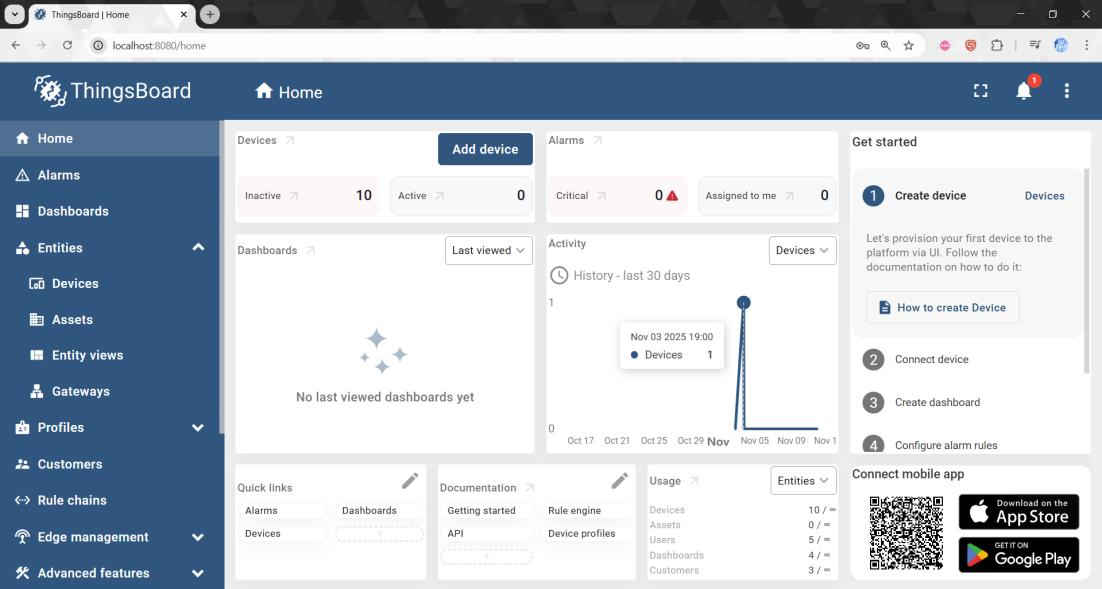
\includegraphics[width=0.92\linewidth,keepaspectratio]{gambar/gambar_2_3.png}
  \caption{Tampilan antarmuka platform ThingsBoard Community Edition}
  \label{fig:thingsboard}
\end{figure}

Sistem \textit{widget} ThingsBoard berbasis \textit{telemetry key} memungkinkan
setiap \textit{field} dalam payload JSON dari perangkat dipetakan ke komponen
visualisasi yang sesuai tanpa memerlukan pemrograman \textit{frontend}.
Contohnya adalah \textit{value card} untuk BPM, \textit{status badge} berwarna
untuk hasil klasifikasi, dan \textit{time-series chart} untuk tren laju jantung.
ThingsBoard juga menyediakan \textit{alarm rule engine} yang dapat dikonfigurasi
untuk memicu notifikasi otomatis ketika kondisi tertentu terpenuhi, misalnya
ketika label = 1 (Aritmia terdeteksi). Dalam penelitian ini, ThingsBoard CE
\textit{self-hosted} digunakan sebagai \textit{broker} MQTT sekaligus
\textit{dashboard} pemantauan hasil klasifikasi dari ESP32-S3.

\subsection{MIT-BIH \textit{Arrhythmia Database}}
\label{subsec:mitbih}

% NOTE: sloppypar dipakai karena "elektrokardiogram" bikin overfull hbox
\begin{sloppypar}
MIT-BIH \textit{Arrhythmia Database} merupakan basis data rekaman
elektrokardiogram standar yang dikembangkan melalui kolaborasi antara
Massachusetts Institute of Technology dan Beth Israel Hospital (BIH) sejak
awal tahun 1980-an. Basis data ini berisi 48 rekaman ECG dua kanal dari
47 subjek, masing-masing berdurasi sekitar 30 menit, yang dicuplik pada
frekuensi 360 Hz dengan resolusi 11-bit pada rentang $\pm$5 mV. Kanal
utama yang digunakan adalah modifikasi sadapan Lead II (MLII), yang
merupakan kanal yang sama dengan konfigurasi sensor pada penelitian
ini~\cite{moody_mark_2001}.
\end{sloppypar}

Keseluruhan rekaman telah dianotasi secara manual oleh kardiolog ahli,
menandai lokasi dan jenis setiap detak jantung. Anotasi ini menggunakan
sistem simbol standar AAMI (\textit{Association for the Advancement of
Medical Instrumentation}) yang mencakup lebih dari 15 jenis detak.
Di antaranya terdapat detak sinus normal (N), kontraksi ventrikular
prematur (V), dan detak supraventrikular (S). Tingkat anotasi per-detak inilah yang
menjadikan MIT-BIH sebagai \textit{benchmark} utama untuk evaluasi
algoritma deteksi aritmia secara global~\cite{moody_mark_2001}. Contoh rekaman beserta anotasinya ditunjukkan pada Gambar~\ref{fig:mitbih-ecg}.

\begin{figure}[H]
  \centering
  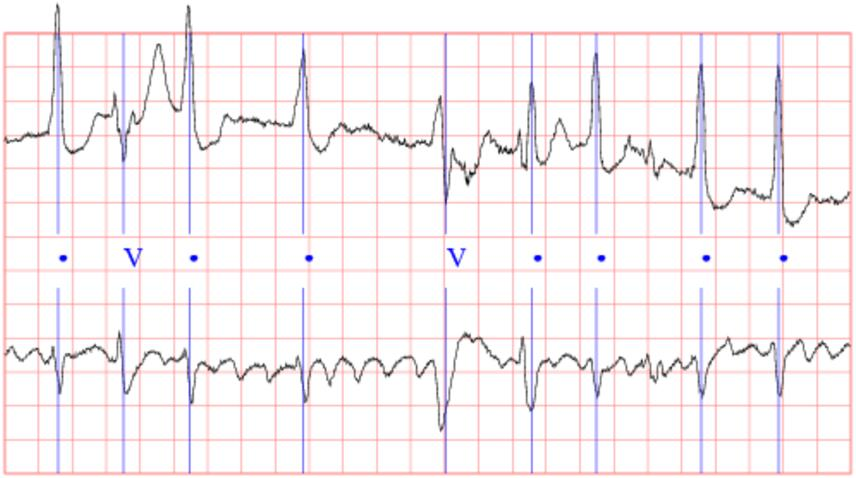
\includegraphics[width=0.90\linewidth,keepaspectratio]{gambar/gambar_2_4.png}
  \caption{Contoh visualisasi rekaman ECG dua kanal dari MIT-BIH
           \textit{Arrhythmia Database} beserta anotasi per-detak,
           dengan simbol ``V'' menunjukkan kontraksi ventrikular prematur (PVC)
           dan simbol titik menunjukkan detak normal}
  \label{fig:mitbih-ecg}
\end{figure}

Dalam penelitian ini, MIT-BIH \textit{Arrhythmia Database} digunakan
sebagai sumber data untuk dua keperluan yang berbeda. Model CNN dilatih
dengan rekaman dari separuh kelompok pasien (DS1) dan diuji dengan rekaman
dari kelompok pasien yang berbeda sepenuhnya (DS2), yang dikenal sebagai
pembagian \textit{inter-patient}.
Strategi ini memastikan bahwa performa model yang diukur mencerminkan
kemampuan generalisasi terhadap pasien baru yang tidak pernah dilihat
selama pelatihan, dan bukan sekadar hafalan pola dari pasien yang sama.

\subsection{Simulasi \textit{Error} Deteksi R-\textit{peak} dengan \textit{Jitter}}
\label{subsec:augmentasi-jitter}

Klasifikasi per detak memotong sinyal ECG menjadi \textit{window} di sekitar puncak R. Pada MIT-BIH posisi tersebut berasal dari anotasi kardiolog, sedangkan pada perangkat posisi itu dihasilkan detektor R-\textit{peak} yang dapat meleset, sehingga evaluasi dengan posisi anotasi belum mewakili pemakaian nyata~\cite{dias_2021}. Dias et al.~\cite{dias_2021} mensimulasikan \textit{error} tersebut dengan \textit{jitter}, yaitu menggeser setiap puncak R menjadi $r'_i = r_i + u_i$. Nilai $u_i$ diambil acak dari sebaran seragam pada rentang $\pm\delta$ sampel, lalu \textit{window} dipotong dan fitur R-R dihitung dari posisi baru. Batas $\delta = 18$ sampel setara dengan toleransi \textit{error} 50 ms pada studi kinerja detektor QRS. Pada batas tersebut, sensitivitas kelas N, S, dan V hanya turun dari 94,5\%, 92,5\%, dan 88,6\% menjadi 93,7\%, 89,7\%, dan 87,9\%~\cite{dias_2021}.
% sumber: Dias 2021 (CMPB 202:105948) sec. 4.2 hlm. 3 (uniform -delta..+delta, delta 0..18, 18 sampel = 50 ms, 128+127 sampel), sec. 4.3.1 (RR dari posisi tersegmentasi), sec. 5.2 hlm. 6 (33 ulangan), Tabel 3 hlm. 5 (Se N/S/V delta 0: 94,5/92,5/88,6; delta 18: 93,7/89,7/87,9)

Dias et al.\ memakai \textit{jitter} sebagai uji ketahanan. Dalam penelitian ini, \textit{jitter} dipakai sebagai augmentasi data latih dengan dua penyesuaian. Besar pergeseran diambil ulang dari sebaran \textit{error} detektor yang diukur sendiri pada DS1, karena sekitar 80\% deteksi hanya berselisih satu sampel atau kurang dari anotasi, sedangkan sebagian kecil lainnya menyimpang hingga puluhan sampel. Selain itu, setiap detak DS1 disertai salinan ber-\textit{jitter} di samping salinan bersihnya, sedangkan DS2 dibiarkan bersih sebagai data uji.
% sumber: model/docs/jitter-walkthrough.md bagian 2 (DS1 50.601 pasangan, 79,85% <=1 sampel, |p99| 26, maks 54); model/config.py (JITTER_MODEL = "empiris", JITTER_SALINAN = 2); model/scripts/prep_beats.py (1 bersih + 2 jitter, hanya DS1 mitdb)

\section{Penelitian Terkait}
\label{sec:penelitian-terkait}

\subsection{A Multistage Denoising Framework for Ambulatory ECG Signal Based on Domain Knowledge and Motion Artifact Detection}
\label{subsec:related-xie2021}

Xie et al.~\cite{xie_2021} mengusulkan kerangka preprocessing multi-tahap untuk sinyal ECG \textit{ambulatory}. Kerangka tersebut menggabungkan \textit{Frequency-Adaptive Noise Estimation} (FANE) berbasis \textit{wavelet} untuk menekan \textit{motion artifact}, \textit{Morphological Analysis and Detection} (MAD), \textit{Singular Value Thresholding} (SVT), serta \textit{Complete Ensemble Empirical Mode Decomposition} (CEEMD) untuk mengatasi \textit{baseline wander}. Kombinasi metode ini terbukti meningkatkan \textit{Signal-to-Noise Ratio} (SNR) sebesar 7\%--25\% dibandingkan metode konvensional pada \textit{dataset} ECG \textit{ambulatory}. Namun, seluruh eksperimen dilakukan pada perangkat PC server tanpa pelaporan latensi pemrosesan atau penggunaan memori. Penelitian tersebut memberikan referensi penting untuk memahami tantangan \textit{noise} pada ECG \textit{ambulatory}, sekaligus menunjukkan \textit{gap} bahwa algoritma preprocessing yang efektif belum divalidasi pada MCU \textit{low-power}.

Berbeda dengan penelitian tersebut yang menumpukan penekanan \textit{noise} pada CEEMD dan \textit{wavelet} yang beban komputasinya berat dan belum dikuantisasi untuk mikrokontroler, penelitian ini memakai filter Butterworth dan deteksi R-\textit{peak} Pan-Tompkins yang ringan. Pilihan itu diambil agar preprocessing dapat berjalan \textit{real-time} pada mikrokontroler hemat daya dan beban komputasinya terukur.

\subsection{A Real-Time Embedded System to Detect QRS-Complex and Arrhythmia Classification Using LSTM Through Hybridized Features}
\label{subsec:related-karri2023}

Karri dan Annavarapu~\cite{karri_2023} merancang sistem \textit{embedded} \textit{real-time} untuk deteksi kompleks QRS dan klasifikasi aritmia menggunakan pendekatan \textit{hybrid} yang menggabungkan \textit{Discrete Wavelet Transform} (DWT), \textit{Delta-Sigma Modulation} (DSM), dan model LSTM. Sistem DWT+DSM mampu mendeteksi kompleks QRS dalam 17,2 ms dengan konsumsi daya 680 nW pada chip DSM, dan diuji pada Raspberry Pi 4 (ARM Cortex-A72, RAM 4 GB). Meskipun berhasil menunjukkan kelayakan pemrosesan ECG secara \textit{embedded}, penggunaan Raspberry Pi 4 tidak mewakili batasan MCU \textit{low-power} yang sesungguhnya. \textit{Gap} pada penelitian tersebut adalah absennya implementasi dan validasi pada MCU kelas ESP32 atau Cortex-M4.

Berbeda dengan penelitian tersebut yang tidak mengukur daya total maupun RAM dan belum terhubung ke \textit{cloud}, penelitian ini menjalankan seluruh jalur pada mikrokontroler ESP32-S3 dan melaporkan beban komputasi serta memori yang terpakai di perangkat. Hasil klasifikasinya kemudian diteruskan ke \textit{cloud} melalui MQTT.

\subsection{Real-Time Fetal Arrhythmia Detection Using Deep Learning on an Embedded fECG Monitoring System}
\label{subsec:related-mekhfioui2025}

Mekhfioui et al.~\cite{mekhfioui_2025} mengembangkan sistem deteksi aritmia jantung janin berbasis sinyal fECG. Sistem tersebut memakai \textit{Independent Component Analysis} (ICA) untuk separasi sinyal, diikuti \textit{bandpass filtering} dan segmentasi ke dalam jendela 3 detik, serta klasifikasi menggunakan model 1D-CNN ringan yang diimplementasikan pada Raspberry Pi. Sistem mencapai akurasi 98,2\%, sensitivitas 98,8\%, dan F1-\textit{score} 98,1\% pada \textit{dataset} Kaggle dan NIFECGDB. Penelitian tersebut menjadi acuan arsitektur 1D-CNN untuk klasifikasi sinyal kardiovaskular pada \textit{embedded system}. Namun, implementasinya masih pada Raspberry Pi, dan ICA belum dievaluasi pada MCU dengan batasan RAM dan daya yang jauh lebih ketat.

Berbeda dengan penelitian tersebut yang memakai ICA yang sensitif terhadap \textit{noise}, penelitian ini memakai jalur preprocessing deterministik yang beban komputasinya diukur langsung di mikrokontroler.

\subsection{TinyML-Based Classification in an ECG Monitoring Embedded System}
\label{subsec:related-kim2023}

Kim et al.~\cite{kim_2023} mengusulkan TinyCES, sebuah model 1D-CNN terkuantisasi yang dirancang khusus untuk monitoring ECG pada perangkat \textit{embedded} dengan sumber daya terbatas. Model berhasil di-\textit{deploy} pada Arduino Nano 33 BLE Sense (ARM Cortex-M4) dengan ukuran model 27 KB dan akurasi klasifikasi biner sebesar 97\% menggunakan \textit{dataset} MIT-BIH dan PTB ECG. Penelitian tersebut merupakan salah satu dari sedikit studi yang benar-benar menjalankan inferensi ECG di MCU fisik \textit{low-power}. Namun, TinyCES masih terbatas pada klasifikasi biner dan tidak menyertakan laporan latensi inferensi, penggunaan RAM saat \textit{runtime}, maupun konsumsi daya aktual selama operasi kontinu.

Penelitian tersebut paling dekat dengan pendekatan penelitian ini. Berbeda dengan penelitian tersebut yang berhenti pada inferensi di perangkat, penelitian ini melengkapi inferensi INT8 di ESP32-S3 dengan pengukuran latensi dan memori di perangkat serta \textit{pipeline} \textit{edge-to-cloud} yang resilien, sedangkan klasifikasinya sama-sama biner.

\subsection{Designing Resilient IoT and Edge Computing with Federated TinyML}
\label{subsec:related-laiu2026}

Laiu et al.~\cite{laiu_2026} mengusulkan arsitektur DRIFT (\textit{Distributed Resilient IoT Federated TinyML}), sebuah kerangka tiga-lapisan yang mengintegrasikan TinyML dan \textit{Federated Learning} untuk meningkatkan keamanan dan ketahanan sistem IoT/MCU. Penelitian tersebut menunjukkan bahwa kuantisasi float32 ke INT8 menghasilkan kompresi model $4\times$ dengan degradasi akurasi kurang dari $0{,}01\%$, serta membuktikan bahwa beban komputasi pada MCU dapat dikurangi melalui preprocessing terdistribusi di lapisan \textit{edge}. Fokus penelitian tersebut adalah pada keamanan siber IoT, bukan pada monitoring sinyal biomedis, dan evaluasinya dilakukan secara simulasi tanpa pengujian \textit{streaming} data ECG kontinu pada \textit{hardware} MCU fisik.

Berbeda dengan penelitian tersebut yang mengevaluasi kuantisasi pada deteksi intrusi jaringan secara simulasi, penelitian ini menerapkan kuantisasi INT8 pada model deteksi aritmia. Selisih metrik dan latensinya diukur langsung di ESP32-S3 dengan \textit{streaming} ECG kontinu.

\subsection{Implementing TinyML in Internet of Things Devices: A Systematic Literature Review}
\label{subsec:related-solispino2026}

Solis Pino et al.~\cite{tinyml_iot_review} melakukan tinjauan literatur sistematis terhadap 114 studi primer tentang implementasi TinyML pada perangkat IoT menggunakan protokol PRISMA dan strategi pencarian multi-\textit{database}. Hasil \textit{review} mengungkapkan bahwa CNN adalah arsitektur yang paling sering digunakan, ESP32 dan Arduino Nano 33 BLE Sense adalah platform \textit{hardware} yang paling umum, serta \textit{healthcare} adalah domain aplikasi yang paling banyak diteliti. Tinjauan ini juga mengidentifikasi tantangan utama yang belum terselesaikan, meliputi keterbatasan memori/CPU, kerentanan keamanan, dan absennya standardisasi implementasi TinyML antar platform.

Berbeda dengan tinjauan tersebut yang memetakan praktik lintas studi tanpa eksperimen, penelitian ini memakai temuannya sebagai dasar pemilihan CNN, ESP32, dan TFLite Micro, lalu menguji pilihan itu secara eksperimental pada satu perangkat.

\subsection{Advanced IoT-Enabled Embedded Wearable System for Continuous Cardiovascular Health Monitoring Using Edge Intelligence}
\label{subsec:related-sheebarani2026}

Sheeba Rani et al.~\cite{sheeba_rani_2026} mengusulkan sistem \textit{wearable} monitoring kardiovaskular kontinu yang mengimplementasikan model \textit{hybrid} 1D-TA-DSC (kombinasi 1D \textit{Depthwise Separable Convolution} dan \textit{Temporal Attention}-GRU) pada ARM Cortex-M4 menggunakan TFLite. Setelah kuantisasi \textit{post-training}, model dikompres dari 22 KB menjadi 11 KB dengan latensi inferensi 7 ms, akurasi 99,8\%, dan AUROC 0,997 pada \textit{dataset} MIMIC-III (rekaman ICU). Penelitian tersebut adalah salah satu yang paling detail dalam melaporkan metrik \textit{hardware} untuk monitoring kardiovaskular di MCU. Namun, penelitian tersebut tidak menyertakan evaluasi konsumsi daya pada kondisi operasi kontinu maupun mekanisme resiliensi \textit{pipeline} \textit{edge-to-cloud}.

Berbeda dengan penelitian tersebut yang dilatih pada rekaman ICU MIMIC-III yang belum tentu mewakili kondisi \textit{ambulatory}, penelitian ini dilatih dan diuji secara \textit{inter-patient} pada MIT-BIH. Penelitian ini juga menambahkan \textit{pipeline} \textit{edge-to-cloud} yang resilien yang tidak dibahas pada penelitian tersebut.

\subsection{An On-Device Machine Learning Assisted System for Unobtrusive Cardiac Auscultation}
\label{subsec:related-chowdhury2023}

Chowdhury dan Chattopadhyay~\cite{chowdhury_2023} mengembangkan sistem auskultasi jantung berbasis \textit{on-device machine learning} yang diimplementasikan pada Arduino Nano 33 BLE Sense (ARM Cortex-M4, 64 MHz) untuk klasifikasi suara jantung secara \textit{real-time} tanpa koneksi internet. Sistem melaporkan latensi \textit{pipeline} DSP sebesar 23,19 ms untuk ekstraksi fitur MFCC, dengan konsumsi arus puncak 8,6 mA pada 3,3 V (sekitar 28,38 mW) dan daya tahan baterai 11,5 jam menggunakan baterai 240 mAh. Penelitian tersebut memberikan referensi \textit{benchmark} konsumsi daya aktual untuk \textit{inference on-device} pada MCU Cortex-M4, meskipun fokusnya pada auskultasi suara jantung, bukan sinyal ECG.

Berbeda dengan penelitian tersebut yang mengolah suara jantung (PCG), penelitian ini mengolah sinyal ECG dengan jalur inferensi yang serupa di perangkat.

\subsection{AI-Powered Anomaly Detection and Cybersecurity in Healthcare IoT with Fog/Edge}
\label{subsec:related-alquayed2026}

Al-Quayed~\cite{al_quayed_2026} mengusulkan kerangka FE-ACS yang mendistribusikan pemrosesan dan deteksi anomali ke lapisan \textit{fog} dan \textit{edge} pada ekosistem IoT kesehatan. Pengukuran performa menunjukkan bahwa arsitektur \textit{fog-edge} mencapai latensi total rata-rata 18,7 ms dibandingkan 152,3 ms pada arsitektur \textit{cloud-centric}, mempresentasikan peningkatan 87,7\% dengan efisiensi \textit{bandwidth} $8{,}5\times$ lebih tinggi. Penelitian tersebut membuktikan secara kuantitatif keunggulan arsitektur \textit{edge} atas \textit{cloud-centric} untuk aplikasi IoT kesehatan. Namun, fokus penelitian tersebut adalah pada keamanan siber, bukan pada \textit{streaming} data ECG kontinu, dan tidak membahas mekanisme resiliensi saat koneksi terputus.

Berbeda dengan penelitian tersebut yang mengukur keunggulan latensi \textit{fog-edge} untuk deteksi anomali keamanan, penelitian ini memakai bukti kuantitatif itu sebagai dasar pemindahan inferensi ke perangkat. Penelitian ini juga menambahkan mekanisme bufer lokal untuk \textit{streaming} ECG saat koneksi terputus.

\subsection[Resilient Edge-to-Cloud Architecture with Self-Healing and Self-Correcting Mechanisms for Industrial Data Continuity]{Resilient Edge-to-Cloud Architecture with Self-Healing and\\ Self-Correcting Mechanisms for Industrial Data Continuity}
\label{subsec:related-boluda2026}

Boluda-Prieto et al.~\cite{resilient_edge_cloud} mengusulkan arsitektur E2C (\textit{Edge-to-Cloud}) berbasis \textit{microservices} dengan mekanisme \textit{self-healing} dan \textit{self-correcting} menggunakan \textit{stack} Kubernetes, Rancher, Prometheus, Grafana, dan Node-RED. Sistem menggunakan MQTT sebagai protokol transmisi dengan mekanisme \textit{edge buffering} yang mempertahankan \textit{Recovery Point Objective} (RPO) mendekati nol untuk aliran data kritis saat terjadi saturasi jaringan. Pengujian \textit{stress test} dengan kondisi \textit{overload} CPU dan saturasi jaringan menunjukkan kemampuan sistem mendeteksi \textit{threshold}, melakukan \textit{scaling}, dan mengisolasi \textit{node} bermasalah secara otomatis. Meskipun prinsip resiliensi pada penelitian tersebut relevan untuk \textit{streaming} ECG, seluruh implementasi berfokus pada data \textit{time-series} industri manufaktur dan menggunakan infrastruktur berbasis Kubernetes yang terlalu berat untuk MCU \textit{low-power}.

Berbeda dengan arsitektur tersebut yang mengandalkan \textit{microservices} Kubernetes di sisi server, penelitian ini menerapkan prinsip \textit{edge buffering} yang sama di dalam mikrokontroler. \textit{Ring buffer} di PSRAM ESP32-S3 menahan detak saat koneksi terputus dan mengurasnya saat koneksi pulih.

\subsection{Real-Time Cardiac Arrhythmia Classification Using TinyML on
Ultra-Low-Cost Microcontrollers}
\label{subsec:related-zambrano2026}

Zambrano-de la Torre et al.~\cite{zambrano_2026} menunjukkan klasifikasi aritmia \emph{real-time} menggunakan
1D-CNN terkuantisasi INT8 yang di-\emph{deploy} pada mikrokontroler Arduino UNO 8-bit
(ATmega328P, SRAM 2 KB, Flash 32 KB). Sistemnya mengintegrasikan akuisisi sinyal ECG
dengan \emph{front-end} analog AD8232, filter Butterworth \emph{bandpass} 0,5--40 Hz,
deteksi R-peak Pan-Tompkins, segmentasi \emph{window} 250 sampel (sekitar 0,7 detik
pada 360 Hz), hingga visualisasi pada layar OLED. Model dilatih dan dievaluasi pada
MIT-BIH Arrhythmia Database untuk tiga kelas (Normal, Ventrikular, Supraventrikular).
Model yang dihasilkan berukuran di bawah 22 KB dengan latensi inferensi sekitar 200 ms
per detak dan degradasi akurasi kurang dari 0,7\% akibat kuantisasi INT8. Validasi
dilakukan melalui dua jalur terpisah, yaitu evaluasi model pada dataset \emph{benchmark}
dan uji fungsional \emph{real-time} menggunakan relawan sehat tanpa penegakan diagnosis
klinis. Penelitian tersebut memberikan bukti kelayakan bahwa \textit{pipeline}
akuisisi--preprocessing--inferensi INT8 dapat berjalan pada mikrokontroler yang
jauh lebih terbatas dari ESP32-S3. Namun, pembagian datanya dilakukan per-detak tanpa
pemisahan antarpasien, sehingga metriknya berpotensi optimistis.

Berbeda dengan penelitian tersebut yang membagi data per detak dan tidak memakai
cabang ritme, penelitian ini mengadopsi skema antarpasien (\emph{inter-patient},
DS1/DS2) yang lebih ketat untuk mengukur generalisasi. Penelitian ini juga menambahkan
cabang ritme berbasis interval R-R, dan perangkatnya dilengkapi \textit{pipeline}
\textit{edge-to-cloud} yang resilien yang tidak ada pada penelitian tersebut.

\subsection{Rancang Bangun Smart Wearables Terintegrasi IoT untuk Deteksi Dini
Atrial Fibrilasi Menggunakan SVM Berbasis Cloud}
\label{subsec:related-mulyawan2026}

Mulyawan~\cite{mulyawan_2026} merancang perangkat \emph{wearable} berbasis ESP32 yang mengintegrasikan
sensor EKG AD8232, sensor SpO\textsubscript{2} MAX30102, dan sensor suhu MLX90614 untuk
deteksi dini atrial fibrilasi (AFib). Deteksi puncak R dan ekstraksi fitur interval RR
dilakukan di sisi \emph{edge}, kemudian fitur ditransmisikan via MQTT ke infrastruktur
\emph{cloud} lokal berbasis ThingsBoard Community Edition dan basis data PostgreSQL.
Klasifikasi dilakukan oleh model Support Vector Machine (SVM) dengan kernel Radial Basis
Function yang \emph{di-deploy pada sisi backend}, dilatih menggunakan dataset MIT-BIH dan
mencapai akurasi tinggi pada pengujian \emph{offline}.
Gambar~\ref{fig:alat-mulyawan} menampilkan \emph{prototype} perangkat yang dihasilkan.

\begin{figure}[H]
  \centering
  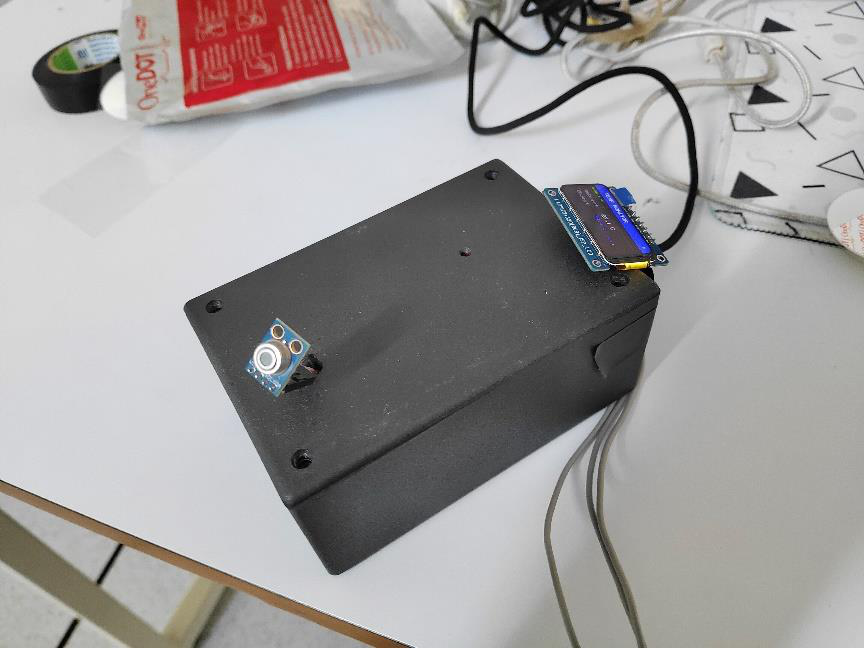
\includegraphics[width=0.7\linewidth]{gambar/gambar_alat_terdahulu_mulyawan.png}
  \caption{\emph{Prototype} perangkat \emph{wearable} pada penelitian
  terdahulu~\cite{mulyawan_2026}, berupa integrasi ESP32 dan sensor AD8232/MAX30102/MLX90614 dalam \emph{blackbox}}
  \label{fig:alat-mulyawan}
\end{figure}

Penelitian tersebut merupakan pendahulu langsung dari penelitian ini dengan platform
sensor dan \emph{dashboard} yang sama, dan penelitian ini melanjutkan rancangan tersebut
pada lokasi inferensi yang berbeda. Berbeda dengan penelitian tersebut yang menjalankan
klasifikasi secara terpusat di \emph{cloud} sehingga pengambilan keputusan tetap
bergantung pada ketersediaan koneksi, penelitian ini memindahkan inferensi sepenuhnya ke
perangkat (\emph{on-device}) menggunakan CNN terkuantisasi INT8. Selain itu, penelitian
ini menambahkan mekanisme resiliensi \emph{pipeline} saat koneksi terputus yang belum
disertakan pada penelitian terdahulu.

\subsection{Perbandingan Penelitian Terkait}
\label{subsec:perbandingan-penelitian}

Berdasarkan ulasan kedua belas penelitian tersebut, Tabel~\ref{tab:perbandingan-penelitian} merangkum perbandingan metode, platform, dan perbedaan utama setiap penelitian terhadap penelitian ini.

{\scriptsize
\setlength{\tabcolsep}{3pt}
\renewcommand{\arraystretch}{1.2}
\begin{longtable}{|c|L{3.5cm}|L{2.0cm}|L{2.0cm}|L{1.8cm}|L{2.8cm}|}
\caption{Perbandingan Penelitian Terkait}\label{tab:perbandingan-penelitian}\\
\hline
\textbf{No} & \textbf{Judul (Tahun)} & \textbf{Penyakit / Domain} & \textbf{Metode (Model)} & \textbf{Platform Komputasi} & \textbf{Perbedaan} \\ \hline
\endfirsthead
\hline
\textbf{No} & \textbf{Judul (Tahun)} & \textbf{Penyakit / Domain} & \textbf{Metode (Model)} & \textbf{Platform Komputasi} & \textbf{Perbedaan} \\ \hline
\endhead
\endfoot
\endlastfoot

1 & \textit{A multi-stage denoising framework for ambulatory ECG signal based on domain knowledge and motion artifact detection} (2021) & Preprocessing sinyal ECG (penekanan noise) & FANE+MAD, SVT, CEEMD, wavelet (denoising bertingkat) & PC server (offline) & \textit{Denoising} bertingkat efektif (SNR naik 7--25\%), tetapi hanya dievaluasi di PC server dan belum diuji pada mikrokontroler. \\ \hline

2 & \textit{A real-time embedded system to detect QRS-complex and arrhythmia classification using LSTM through hybridized features} (2023) & Aritmia & DWT + Delta-Sigma Modulation + LSTM & Raspberry Pi 4 & Akurasi 99,6\% dan \textit{real-time} di Raspberry Pi 4, yang bukan MCU \textit{low-power}, tanpa integrasi \textit{cloud}. \\ \hline

3 & \textit{Real-time fetal arrhythmia detection using deep learning on an embedded fECG monitoring system} (2025) & Aritmia janin (\textit{fetal}) & Bandpass + ICA + 1D-CNN ringan & Raspberry Pi 4 & 1D-CNN ringan dengan transmisi Wi-Fi di Raspberry Pi, ICA belum dievaluasi di MCU dan daya tidak dilaporkan. \\ \hline

4 & \textit{TinyML-Based Classification in an ECG Monitoring Embedded System} (2023) & Aritmia (klasifikasi biner normal/\allowbreak abnormal) & 1D-CNN INT8 (TFLM, \textit{Post-Training Quantization}) & Arduino Nano BLE (Cortex-M4) & Inferensi \textit{on-device} INT8 (\textasciitilde27 KB, akurasi \textasciitilde97\%), terdekat dengan pendekatan ini, tetapi tanpa laporan latensi, daya, dan \textit{pipeline} resilien. \\ \hline

5 & \textit{Designing resilient IoT and Edge Computing with federated TinyML} (2026) & --- (keamanan jaringan IoT) & \textit{Federated Learning} + kuantisasi MLP INT8 & Testbed/\allowbreak simulasi & Kuantisasi float32$\rightarrow$INT8 (kompresi 4$\times$, akurasi turun $<$0,01\%) pada deteksi intrusi jaringan, tanpa \textit{benchmark} MCU fisik. \\ \hline

6 & \textit{Implementing TinyML in Internet of Things devices: A systematic literature review} (2026) & --- (tinjauan literatur, 114 studi) & SLR (PRISMA) & Berbagai (MCU + SBC) & Tinjauan literatur, bukan eksperimen, memetakan algoritma, \textit{hardware}, dan tantangan TinyML (memori, CPU, standardisasi). \\ \hline

7 & \textit{Advanced IoT-enabled embedded wearable system for continuous cardiovascular health monitoring using edge intelligence} (2026) & Penyakit kardio\-vaskular / aritmia (4 kelas keparahan) & 1D Depthwise-\allowbreak Separable Conv + Temporal Attention-\allowbreak GRU (INT8 PTQ) & ARM Cortex-M4 (STM32\-F407) & Inferensi \textasciitilde7 ms dengan model \textasciitilde11 KB di Cortex-M4, tetapi dilatih pada data ICU (MIMIC-III) dan tanpa \textit{pipeline} resilien. \\ \hline

8 & \textit{An on-device machine learning assisted system for unobtrusive cardiac auscultation} (2023) & Kelainan jantung (auskultasi/\allowbreak PCG) & DSP + MFCC + ML \textit{on-device} & Arduino Nano BLE & Berhasil menjalankan ML \textit{on-device}, tetapi memproses sinyal suara jantung (PCG), bukan sinyal ECG. \\ \hline

9 & \textit{AI-Powered Anomaly Detection and Cybersecurity in Healthcare IoT with Fog/Edge} (2026) & Keamanan siber IoT kesehatan & Kerangka FE-ACS (deteksi anomali \textit{fog-edge}) & Arsitektur \textit{fog/edge} IoT & Latensi \textit{fog-edge} 18,7 ms vs 152,3 ms \textit{cloud-centric}, tetapi berfokus keamanan siber, tanpa resiliensi putus koneksi. \\ \hline

10 & \textit{Resilient Edge-to-Cloud Architecture with Self-Healing and Self-Correcting Mechanisms for Industrial Data Continuity} (2026) & Kontinuitas data industri & E2C \textit{microservices} + MQTT + \textit{edge buffering} (\textit{self-healing}) & Kubernetes (Rancher, Prometheus, Grafana) & RPO mendekati nol saat saturasi jaringan, tetapi untuk data industri dengan Kubernetes yang terlalu berat bagi MCU. \\ \hline

11 & \textit{Real-Time Cardiac Arrhythmia Classification Using TinyML on Ultra-Low-Cost Microcontrollers} (2026) & Aritmia (3 kelas: N/V/S) & 1D-CNN INT8 (TFLM, PTQ) + AD8232 & Arduino UNO 8-bit (ATmega328P) & Jalur AD8232 ke inferensi INT8 (model $<$22 KB) berjalan di MCU 8-bit, tetapi data dibagi per detak, tanpa \textit{pipeline} resilien. \\ \hline

12 & \textit{Rancang Bangun Smart Wearables Terintegrasi IoT untuk Deteksi Dini Atrial Fibrilasi Menggunakan SVM Berbasis Cloud} (2026) & Atrial fibrilasi & Fitur RR + SVM (RBF) & ESP32 (akuisisi) + SVM di cloud & Pendahulu langsung dengan sensor dan \textit{dashboard} sama, tetapi inferensi di \textit{cloud}, tanpa kuantisasi di MCU maupun resiliensi \textit{pipeline}. \\ \hline

13 & \textit{Implementasi Sistem Monitoring Detak Jantung Kontinu Berbasis IoT Edge Computing untuk Deteksi Dini Aritmia} (penelitian ini) & Aritmia (deteksi dini) & Preprocessing di MCU (Butterworth + Pan-Tompkins) + 1D-CNN INT8 + fitur RR (\textit{hybrid}) \textit{on-device} ($\pm$23 KB) & \textit{ESP32-S3 (inferensi on-device)} & Preprocessing \textit{real-time}, inferensi CNN INT8, dan \textit{pipeline} resilien (\textit{ring buffer} lokal + MQTT) menyatu dalam satu ESP32-S3. \\ \hline
% sumber: model/artifacts/metrics/fase7_delta.csv (ukuran_kb 22.94)

\end{longtable}
}

Tabel~\ref{tab:perbandingan-penelitian} memperlihatkan bahwa belum ada penelitian yang menyatukan ketiga aspek sekaligus. Ketiga aspek itu adalah preprocessing ECG yang divalidasi di MCU \textit{low-power}, inferensi TinyML \textit{on-device}, serta \textit{pipeline} \textit{edge-to-cloud} dengan resiliensi berbasis MQTT dan bufer lokal. Kelompok pertama mengevaluasi metodenya di PC server atau secara simulasi, yaitu kerangka \textit{denoising} multi-tahap~\cite{xie_2021} dan kuantisasi pada deteksi intrusi~\cite{laiu_2026}, sehingga beban komputasi dan memorinya di mikrokontroler belum diketahui. Kelompok kedua sudah berjalan di perangkat \textit{embedded}, tetapi memakai Raspberry Pi~\cite{karri_2023} atau infrastruktur Kubernetes~\cite{resilient_edge_cloud} yang jauh lebih berat daripada MCU, atau berhenti pada inferensi di MCU tanpa \textit{pipeline} \textit{edge-to-cloud} yang resilien~\cite{kim_2023}.

Penelitian ini memilih ESP32-S3 sebagai satu perangkat yang menjalankan preprocessing, inferensi CNN INT8, dan bufer lokal MQTT. Pilihan itu disadari membawa keterbatasan, yaitu klasifikasi biner, uji \textit{pipeline} dengan sumber sinyal \textit{replay}, dan subjek sehat non-klinis. Angka akurasi pada sebagian penelitian tersebut juga tidak dapat dibandingkan secara langsung dengan hasil penelitian ini. Zambrano-de la Torre et al.\ membagi data per detak tanpa pemisahan antarpasien sehingga metriknya berpotensi optimistis~\cite{zambrano_2026, xiao_2023}, sedangkan penelitian pendahulu menyasar deteksi atrial fibrilasi dan melaporkan akurasi pada pengujian \textit{offline}~\cite{mulyawan_2026}. Penelitian ini menggunakan skema \textit{inter-patient} dengan metrik \textit{recall}, \textit{precision}, \textit{specificity}, F1, dan AUC. Kontribusinya karena itu bukan akurasi yang lebih unggul, melainkan evaluasi yang lebih ketat terhadap generalisasi pada pasien baru beserta kinerja yang terukur di perangkat.
